\documentclass[a4paper,12pt]{article}

% --- LANGUAGE & FONT ---
\usepackage{vntex}
\usepackage[english]{babel}
\usepackage{amsmath, amssymb}

% --- PAGE & TEXT LAYOUT ---
\usepackage{a4wide}
\usepackage{geometry}
\geometry{a4paper, left=2cm, right=2cm, top=2.5cm, bottom=4.2cm, footskip=12mm}
\usepackage{setspace}
\usepackage{multicol}
\usepackage{enumitem}

% --- GRAPHICS & TABLES ---
\usepackage{graphicx}
\usepackage{epsfig}
\usepackage{svg}
\usepackage{tikz}
\usetikzlibrary{arrows,snakes,backgrounds,positioning,shapes,calc,fit}
\usepackage{booktabs}
\usepackage{multirow}
\usepackage{tabularx}
\usepackage{makecell}
\usepackage{array}
\usepackage[skip=5pt]{caption}
\usepackage{placeins}
\usepackage{float}       % added: the template uses [H]
\usepackage{longtable}   % added: long tables across pages

% --- COLOURS & CODE ---
\usepackage{color}
\usepackage{xcolor}
\usepackage{colortbl}    % added: coloured table rows
\usepackage{minted}
\usepackage{listings}
\usepackage{algorithm}
\usepackage{algpseudocode}
\usepackage[framemethod=tikz]{mdframed}

% --- HEADER & FOOTER ---
\usepackage{fancyhdr}
\usepackage{lastpage}

% --- HYPERREF (always load last) ---
\usepackage{hyperref}
\hypersetup{urlcolor=blue,linkcolor=black,citecolor=black,colorlinks=true}

% ================= COLOURS =================
\setlength{\columnseprule}{1pt}
\def\columnseprulecolor{\color{black}}
\definecolor{p1}{RGB}{52,101,164}
\definecolor{p2}{RGB}{78,154,6}
\definecolor{p3}{RGB}{204,0,0}
\definecolor{p4}{RGB}{117,80,123}
\definecolor{p5}{RGB}{193,125,17}
\definecolor{p6}{RGB}{32,128,128}
\definecolor{p7}{RGB}{90,90,90}
\definecolor{p8}{RGB}{170,60,120}

% ================= HEADER/FOOTER =================
\everymath{\color{blue}}
\setlength{\headheight}{40pt}
\pagestyle{fancy}
\fancyhead{}
\fancyhead[L]{
 \begin{tabular}{rl}
    \begin{picture}(25,15)(0,0)
    \put(0,-8){
\includegraphics[width=8mm, height=8mm]{hcmut.png}}
   \end{picture}&
    \begin{tabular}{l}
        \textbf{\ttfamily Ho Chi Minh City University of Technology - VNU-HCM}\\
        \textbf{\ttfamily Faculty of Computer Science and Engineering}
    \end{tabular}
 \end{tabular}
}
\fancyhead[R]{}
\fancyfoot{}
\fancyfoot[L]{\scriptsize \ttfamily \textcolor{blue}{Builders Buildathon 2026 - P3 CAD De-ID \\ Team HCMUT TMT, November 2026}}
\fancyfoot[R]{\scriptsize \ttfamily Page {\thepage}/\pageref{LastPage}}
\renewcommand{\headrulewidth}{0.3pt}
\renewcommand{\footrulewidth}{0.3pt}

\setcounter{secnumdepth}{4}
\setcounter{tocdepth}{3}

% ================= COLOURED BOXES =================
% \partbox{color}{title}{content}: short box, no page break
\newcommand{\partbox}[3]{%
\begin{mdframed}[nobreak=true,linecolor=#1,linewidth=1.2pt,topline=false,rightline=false,bottomline=false,leftmargin=0pt,rightmargin=0pt,innerleftmargin=10pt,backgroundcolor=#1!6]
\textbf{\color{#1}#2}\par\smallskip #3
\end{mdframed}}
% \longbox{color}{title}{content}: long box, may break across pages
\newcommand{\longbox}[3]{%
\begin{mdframed}[linecolor=#1,linewidth=1.2pt,topline=false,rightline=false,bottomline=false,leftmargin=0pt,rightmargin=0pt,innerleftmargin=10pt,backgroundcolor=#1!6]
\textbf{\color{#1}#2}\par\smallskip #3
\end{mdframed}}
% \metabox{color}{workload}{prerequisites}{foundation for}{people}
\newcommand{\metabox}[5]{%
\begin{mdframed}[nobreak=true,linecolor=#1,linewidth=1pt,leftmargin=0pt,rightmargin=0pt,backgroundcolor=#1!15]
\textbf{Workload:} #2\par
\textbf{Prerequisites:} #3\par
\textbf{Foundation for:} #4\par
\textbf{People:} #5
\end{mdframed}}

% ================= HELPER MACROS (added for this report) =================
% \trial{...}: trial-run figure, not an official result
\newcommand{\trial}[1]{\textcolor{p5}{\textbf{[trial run]}~#1}}
% \src{...}: source of a figure
\newcommand{\src}[1]{{\footnotesize\textcolor{p7}{(source: #1)}}}
\newcommand{\fn}[1]{\texttt{\detokenize{#1}}}
\newcolumntype{L}[1]{>{\raggedright\arraybackslash}p{#1}}
\newcolumntype{C}[1]{>{\centering\arraybackslash}p{#1}}
\newcolumntype{Y}{>{\raggedright\arraybackslash}X}
\setlist{itemsep=1pt,topsep=2pt}
\renewcommand{\arraystretch}{1.15}

\begin{document}

\begin{titlepage}
\begin{center}
\Large Vietnam National University Ho Chi Minh City \\
\Large Ho Chi Minh City University of Technology \\
\Large Faculty of Computer Science and Engineering
\end{center}

\vspace{1cm}
\begin{center}

\includegraphics[width=4cm]{hcmut.png}
\end{center}
\vspace{1cm}

\begin{center}
\begin{tabular}{c}
    \textbf{\Large BUILDERS BUILDATHON 2026} \\[0.2cm]
    \textbf{\Large (Problem 3)} \\
    ~~\\
    \hline
    \\
    \multicolumn{1}{l}{\textbf{{\Large Problem overview}}}\\
    \\
    \textbf{{\LARGE Machina -- CAD De-ID}}\\[0.2cm]
    {\large De-identifying 139.7 GB of engineering files that stay usable}\\
    \\
    \hline
\end{tabular}
\end{center}

\vspace{0.5cm}

\begin{table}[h]
\centering
\begin{tabular}{rrl}
\hspace{2cm} & Track: & Machina - CAD De-ID \\
& Team: & HCMUT TMT\\
& Student: & Dang Minh Triet - 2510249 \\
& Deadline: & 23:00 Sunday 22/11/2026 (GMT+7) \\
\end{tabular}
\end{table}

\vfill
\begin{center}
{\footnotesize Ho Chi Minh City, November 2026}
\end{center}
\end{titlepage}

\thispagestyle{fancy}
\newpage
\tableofcontents
\newpage

\sloppy

\section{Overview}

\subsection{General information}
\begin{table}[H]
\centering\small
\begin{tabularx}{\textwidth}{L{4.0cm}Y}
\toprule
\textbf{Item} & \textbf{Details} \\
\midrule
Track & Machina -- CAD De-ID (sponsor Machina, \$5{,}000 prize, \textbf{only 12 teams} on the board at the time of the screenshot). Machina refers the \textbf{top 3} teams to a first-round interview for an Engineering Researcher role \\
Problem & An engineering corpus of 188,722 files, 139.7 GB (PDFs, drawings, SolidWorks, Inventor, neutral CAD formats, images, archives). Build a pipeline that replaces identifying information with consistent pseudonyms, while every engineering file stays usable and the links between files stay intact \\
Deadline & \textbf{23:00 Sunday 22/11/2026 (GMT+7)}. The leaderboard at the cutoff is final; nothing new is graded after it \\
Submission limit & \textbf{20 scored attempts} in total, at most 2 per hour, only one submission grading at a time per team. Grading usually takes under 20 minutes once started, at most 3 hours \\
Getting the input & No AWS account needed: download from \url{https://machina-input.joinbuilders.org} with \fn{get-input.sh} (supports \fn{--limit}, \fn{--prefix}, \fn{--jobs}, resumable) or read \fn{manifest.tsv}. Needs a \emph{case-sensitive} filesystem. On a slow connection, rent a VM with at least 400 GB of disk \\
How to submit & One \fn{attempt-N/} folder per attempt with \fn{corpus/}, \fn{code/}, \fn{README.txt}; upload with \fn{upload.py} (1-hour token) to \fn{gs://builders-machina-submissions-1120/}\allowbreak\fn{teams/<team-id>/attempt-N/}, then paste that location into the form. Submitting from your own S3 bucket in us-west-2 is also possible (bucket policy in \fn{challenge.pdf}) \\
Submission limits & \fn{corpus/} at most 400,000 objects; files over 2 GB are skipped during grading; the scorer stops if finding the files it checks takes more than 12 GB of downloads or 1 hour of reading. Files in the Builders folder are deleted 10 days after upload \\
\bottomrule
\end{tabularx}
\caption{General information for P3 \src{track page, challenge.pdf, upload.py}}
\end{table}

\begin{mdframed}[linecolor=orange,linewidth=1pt,backgroundcolor=orange!8]
\textbf{The track page and \fn{challenge.pdf} differ:} the PDF says ``up to three attempts'', copying into your own S3 bucket with the AWS CLI and emailing the location to the organiser. The page says explicitly: ``Where challenge.pdf and this page differ on attempts, where the input comes from, or how to submit, this page applies''. So: \textbf{20 attempts}, download from \fn{machina-input.joinbuilders.org}, submit through the form on the page.
\end{mdframed}

\subsection{Scoring and how it is graded}
P3 is \textbf{graded automatically} by 1,000 private checks. There is no AI or human grading in the score; the organisers may re-grade all teams with a stricter grader during the event, and the board and final ranking use the latest scores.

\begin{table}[H]
\centering\small
\begin{tabularx}{\textwidth}{L{3.3cm}YC{1.9cm}C{1.5cm}}
\toprule
\textbf{Component} & \textbf{Definition} & \textbf{Graded by} & \textbf{Part} \\
\midrule
Attempt score & Checks passed out of 1,000 private checks on \fn{corpus/}: names replaced consistently everywhere they appear, and engineering files still usable & auto & 3.2--3.5 \\
Feedback & Total score and pass counts per \emph{category}; never which checks or files & auto & 3.6 \\
Broken/missing files & A check on a file the scorer cannot find or open fails (and shows as ``not checked''). Keep each file's extension and the non-identifying parts of its path so the scorer can find it & auto & 3.4, 3.5 \\
Rejected (no attempt used) & Malformed location, \fn{corpus/} missing or empty, S3 bucket outside us-west-2 or not publicly readable, over 400,000 objects, over 12 GB of downloads/1 hour of reading & auto & 3.5 \\
Ties & The earlier attempt ranks first & auto & 3.6 \\
\bottomrule
\end{tabularx}
\caption{P3 rubric \src{track page}}
\end{table}

\begin{table}[H]
\centering\small
\begin{tabular}{rlr|rlr}
\toprule
\textbf{Rank} & \textbf{Team} & \textbf{Score} & \textbf{Rank} & \textbf{Team} & \textbf{Score} \\
\midrule
1 & 67 & 660 & 7 & yoookay & 292 \\
2 & Team-Xero & 417 & 8 & We Asked ChatGPT & 271 \\
3 & Hidden Test Cases & 398 & 9 & whyMiso & 158 \\
4 & sirPeasALot & 374 & 10 & AT & 51 \\
5 & Monsters & 293 & 11 & Lone Gradient & 39 \\
6 & putabuilderon & 292 & 12 & prompt-gods & 1 \\
-- & \textit{Baseline (input copied unchanged)} & \textit{292} & & & \\
\bottomrule
\end{tabular}
\caption{P3 leaderboard snapshot, 21/11}
\end{table}

\begin{mdframed}[linecolor=orange,linewidth=1pt,backgroundcolor=orange!8]
\textbf{How to read the board:} copying the input unchanged already scores 292/1000. So about 29\% of the checks are of the ``file still usable / engineering data intact'' kind, and a plain copy passes all of them. 6 of 12 teams are at 292 or below, meaning their pipelines break more files than the names they replace are worth. \textbf{Rule number 1: never break a file}; when a safe edit is not certain, keep the bytes unchanged and note it in the README. Rank 3 is currently 398: about $+110$ checks over the baseline is enough for the top 3.
\end{mdframed}

\subsection{Sources and conventions for figures}
\begin{itemize}
  \item \textbf{Primary sources:} the track page (screenshot). \fn{challenge.pdf} (3 pages) is used for the technical requirements, except where the page overrides it. The repo has no forum Q\&A yet.
  \item \textbf{For reference:} \fn{upload.py} (16 threads by default, 1 MiB chunks, 4 retries, skips files already present with the same size and MD5 \emph{in the same destination folder}).
  \item No trial figures yet: \fn{machina-input.joinbuilders.org} was not reachable from my working environment (network blocked), so the share of each format is unknown. Step one of 3.1 is to fetch \fn{manifest.tsv} and count.
  \item ``Observed'' figure: the D: drive holding the repo has 272 GB with about 113 GB free (measured on your machine through the desktop connection). That is \textbf{not enough} for the 139.7 GB input + unpacked archives + output.
\end{itemize}

\subsection{Dependency diagram}
\begin{center}
\begin{tikzpicture}[
  box/.style={draw,rounded corners,thick,text width=3.3cm,minimum height=1.2cm,align=center,font=\small},
  ext/.style={draw,dashed,rounded corners,text width=3.6cm,minimum height=1cm,align=center,font=\small,fill=gray!8},
  arr/.style={->,thick,>=stealth},
  lab/.style={font=\scriptsize,fill=white,inner sep=1pt}]
  \node[ext] (c) at (0,2.6) {\textbf{Machine}: VM $\ge$ 400 GB, or WSL2 ext4 + batch processing};
  \node[box,draw=p1,fill=p1!10] (a) at (0,0) {\textbf{3.1} Get the data, survey the corpus};
  \node[box,draw=p2,fill=p2!10] (b) at (5.4,0) {\textbf{3.2} Identity detection, pseudonym table};
  \node[box,draw=p3,fill=p3!10] (d) at (10.8,0) {\textbf{3.3} Per-format processing};
  \node[box,draw=p4,fill=p4!10] (e) at (10.8,-2.8) {\textbf{3.4} Rename files/folders, update references};
  \node[box,draw=p5,fill=p5!10] (f) at (5.4,-2.8) {\textbf{3.5} Validate, package the attempt};
  \node[box,draw=p6,fill=p6!10] (g) at (0,-2.8) {\textbf{3.6} Strategy for 20 attempts};
  \draw[arr] (c) -- (a);
  \draw[arr] (a) -- node[lab,above=2pt]{file list} (b);
  \draw[arr] (b) -- node[lab,above=2pt]{pseudonyms} (d);
  \draw[arr] (d) -- (e);
  \draw[arr] (b) -- node[lab,sloped,above=2pt]{file names} (e);
  \draw[arr] (e) -- (f);
  \draw[arr] (f) -- (g);
  \draw[arr,dashed] (d.north) to[bend right=25] node[lab,above=1pt]{new identities found} (b.north);
  \draw[arr,dashed] (g.north) to[bend left=20] node[lab,left=2pt]{per-category scores} (a.south west);
\end{tikzpicture}
\end{center}
Dashed arrows are loops: processing formats reveals more identities (back to extend the pseudonym table), and per-category feedback after each attempt shows which part to work on next. P3 does not depend on P1, P2 or P4 and \emph{does not need GitHub}, but it uses the most bandwidth and disk, so the download must start early.

\subsection{Repo status}

\begin{table}[H]
\centering\small
\begin{tabularx}{\textwidth}{L{4.2cm}Y}
\toprule
\textbf{Item} & \textbf{Status (read on 21/11, around 11:10)} \\
\midrule
Main repo & \fn{martin-danggg/HCMUT_TMT_Builders_BUILDATHON}, branch \fn{main}, remote \fn{origin} over SSH \\
Latest commit & \fn{55687de} ``Initial commit'', 21/11/2026 10:41:21 +0700, author Triet Dang. This is the only commit \\
Committed files & Only \fn{README.md} (31 bytes, a one-line title) \\
Not committed (untracked) & \fn{p1_Builders/} (2.9 MB), \fn{p2_Databricks/} (5.7 MB), \fn{p3_Machina/} (48 KB), \fn{p4_RWX/} (404 KB): all of it is starter files from the organisers; no solution code yet \\
\fn{reports/} folder & Holds this overview (Vietnamese and English, not committed) \\
Main repo \fn{.gitignore} & Ignores the 3 \fn{submission/} folders (separate repos) and \fn{p3_Machina/submission/} (P3 data must stay private) \\
Separate submission repos (created on GitHub, public) & P1: \fn{martin-danggg/hcmut-tmt-p1-mech-royale} $\rightarrow$ \fn{p1_Builders/submission/}\allowbreak\fn{hcmut-tmt-p1-mech-royale/} (commit \fn{f4e1861})\newline P2: \fn{martin-danggg/hcmut-tmt-p2-shopping-sessions} $\rightarrow$ \fn{p2_Databricks/submission/}\allowbreak\fn{hcmut-tmt-p2-shopping-sessions/} (commit \fn{21cd7e4})\newline P4: \fn{martin-danggg/hcmut-tmt-p4-blast-radius} $\rightarrow$ \fn{p4_RWX/submission/}\allowbreak\fn{hcmut-tmt-p4-blast-radius/} (commit \fn{2a682dc})\newline The starter skeleton is cloned, committed as ``Setup: add requirements'' and pushed to \fn{main} by \fn{tools/setup_submissions.sh} \\
\bottomrule
\end{tabularx}
\caption{Status of the main repo, shared by all 4 problems}
\end{table}

\begin{mdframed}[linecolor=orange,linewidth=1pt,backgroundcolor=orange!8]
\textbf{Submitting through separate repos (decided):} P1, P2 and P4 all require \emph{a public GitHub repository with the \fn{Dockerfile} at the root} of the submitted commit. The main repo is a monorepo (p1--p4 in subfolders), so \textbf{the main repo is never submitted}. Each track has its own public repo, kept locally in \fn{pX_.../submission/hcmut-tmt-pX-.../}; each of those folders is an independent git repo with its own remote, and the main repo ignores them via \fn{.gitignore}. To submit: paste the track repo's link (e.g. \fn{https://github.com/martin-danggg/hcmut-tmt-p4-blast-radius}) into \emph{Public GitHub repository}; leave \emph{Commit} empty to use the newest commit on \fn{main}. Keep the repo public, with every submitted commit, until results are published. P3 needs no GitHub (it is submitted through the team's \fn{gs://} folder).
\end{mdframed}


\begin{table}[H]
\centering\small
\begin{tabularx}{\textwidth}{L{5.3cm}C{1.9cm}Y}
\toprule
\textbf{P3 component} & \textbf{Present?} & \textbf{Note} \\
\midrule
\fn{challenge.pdf} & Yes & 3 pages; some points overridden by the track page \\
\fn{upload.py} & Yes & Python 3, standard library only \\
\fn{get-input.sh}, \fn{manifest.tsv} & No & Download from \url{https://machina-input.joinbuilders.org} \\
Input corpus (139.7 GB) & No & Not for the repo; must stay private \\
Pipeline (\fn{code/}), private pseudonym table & No & The pseudonym table lives \emph{outside} the submission folder \\
Attempt \fn{README.txt} & No & Output of 3.5 \\
\bottomrule
\end{tabularx}
\caption{What P3 already has and what is missing}
\end{table}

\subsection{Assignments and schedule}
Working alone, so the ``reviewer'' column does not apply. Instead of review: every attempt must pass the leak scan and the file-open checks (section 3.5).

\begin{table}[H]
\centering\small
\begin{tabularx}{\textwidth}{C{1cm}L{2.6cm}YC{1.6cm}}
\toprule
\textbf{Part} & \textbf{Owner} & \textbf{Task} & \textbf{Review} \\
\midrule
3.1 & Dang Minh Triet & Prepare the machine, download the corpus, format statistics & -- \\
3.2 & Dang Minh Triet & Identity list, consistent pseudonym generation & -- \\
3.3 & Dang Minh Triet & One processor per format & -- \\
3.4 & Dang Minh Triet & Rename paths, fix cross-file references & -- \\
3.5 & Dang Minh Triet & File-open checks, leak scan, README, upload & -- \\
3.6 & Dang Minh Triet & Attempt order, reading per-category feedback & -- \\
\bottomrule
\end{tabularx}
\caption{P3 assignments}
\end{table}

There are no ``weeks'' or ``tag deadlines'': the only deadline is 23:00 Sunday 22/11. P3 gets 6.5 working hours out of about 25 (26\%), not counting background download and upload time. Estimate (not measured): 139.7 GB at 100 Mbps takes about 3.1 hours each way.

\begin{center}\small
\begin{longtable}{L{1.8cm}L{2.1cm}C{1.3cm}L{10.1cm}}
\toprule \textbf{Day} & \textbf{Time} & \textbf{Track} & \textbf{Task} \\ \midrule\endhead
Sat 21/11 & 11:15--12:00 & Shared & Create 3 separate public repos for P1, P2, P4 (Dockerfile at the root); check Docker/WSL2; P3: fetch the manifest, run \fn{get-input.sh --limit 100} \\
 & 12:00--15:30 & P4 & 4.1 environment + 4.2 coverage map at the pinned commit; 4.3--4.4 selector v1; \fn{make sample}; first submission \\
 & 15:30--18:00 & P1 & 1.1 infrastructure + 1.2 map + 1.3 movement/zone; submit bot v1 \\
 & 18:00--19:00 & -- & Break \\
 & 19:00--22:30 & P2 & 2.1--2.7 correct version: 36/36 fixtures, \fn{check-dev} MATCH; first submission \\
\rowcolor{p3!15} & 22:30--23:30 & P3 & 3.1 survey 100 sample files; start the full corpus download in the background overnight \\
 & 23:30--00:30 & P1 & 1.4 combat v2; submit (scored while sleeping) \\
Sun 22/11 & 00:30--07:30 & -- & Sleep (P3 download keeps running) \\
\rowcolor{p3!15} & 07:30--10:30 & P3 & 3.2--3.5 pipeline v1 on the corpus; upload attempt 1 \\
 & 10:30--12:30 & P2 & 2.8 speed optimisation; submit twice \\
 & 12:30--13:30 & -- & Lunch \\
 & 13:30--15:00 & P4 & 4.5 safety rules + worker-split tuning; submit \\
 & 15:00--18:00 & P1 & 1.5 loot/upgrades + 1.6 A/B loop (about 10 submissions) \\
\rowcolor{p3!15} & 18:00--20:30 & P3 & 3.6 attempts 2--3 based on per-category scores \\
 & 20:30--21:30 & P2 & Final improvements, submit \\
 & 21:30--22:00 & P4 & Final improvements, submit \\
 & 22:00--22:45 & Shared & Lock in: pick the final submission for each track, keep repos public, tag \fn{pX-final} \\
 & 22:45--23:00 & -- & Buffer. All tracks close at 23:00 \\
\bottomrule
\caption{Proposed schedule for all 4 tracks up to the 23:00 Sunday 22/11 deadline (highlighted rows are P3)}
\end{longtable}
\end{center}


\subsection{Choosing the overall approach}
\begin{table}[H]
\centering\small
\begin{tabularx}{\textwidth}{L{3.4cm}YYC{1.7cm}}
\toprule
\textbf{Approach} & \textbf{Pros} & \textbf{Cons} & \textbf{Chosen?} \\
\midrule
\multicolumn{4}{l}{\textit{Machine}} \\
Cloud VM $\ge$ 400 GB & Matches the page's advice; fast network so each attempt downloads/uploads quickly & Costs your own money & \textbf{Yes, if budget allows} \\
Personal machine, WSL2 ext4, batches via \fn{--prefix} & Free & D: has about 113 GB free; NTFS is case-insensitive (must use WSL2's ext4); uploading 140 GB per attempt is slow & Backup \\
\midrule
\multicolumn{4}{l}{\textit{How to replace inside binary files}} \\
\textbf{Same-length byte replacement} (pseudonym exactly as long as the original, both ASCII and UTF-16) & No offset shifts, binary structure intact, file-name references can be fixed in place & Pseudonyms constrained in length; does not work inside compressed streams & \textbf{Yes} \\
Rewrite with format libraries (pikepdf, olefile, ezdxf, zip) & Structurally correct & One library per format; proprietary CAD (SolidWorks, DWG) has no good open library & Yes, for open formats \\
Export to PDF/images and drop the originals & Easy & Forbidden: native files must stay usable & No \\
\bottomrule
\end{tabularx}
\caption{Comparison of approaches for P3}
\end{table}

\textbf{Choice:} standard libraries for open formats + same-length replacement for binary parts, because this keeps the ``file still usable'' points (the 292 baseline) while still replacing names. \textbf{On priorities across tracks:} P3 has the fewest teams and rank 3 needs only about 400 points, so it has the best ``effort per rank'' ratio of the 4 tracks; the bottleneck is download and upload, so decide on the machine in the 22:30--23:30 block on Saturday night and download overnight.

\newpage
\section{Parts of the work}

% ---------------------------------------------------------------
\subsection{3.1 Get the data and survey the corpus}
\partbox{p1}{1. What the task requires}{Download the corpus into \fn{./input/} on a case-sensitive filesystem with room for the 139.7 GB input, unpacked archives and the output. Test with 100 files first (\fn{bash get-input.sh --limit 100}), then download everything. Keep the raw input private; do not publish or share it.}
\partbox{p1}{2. Goal when done}{A machine with enough disk; \fn{manifest.tsv} and a statistics table: file count and size by extension, by top-level folders (levels 1--2), number of duplicates (by hash), number of empty/broken files, number of archives and their nesting depth.}
\partbox{p1}{3. Input data and prerequisite knowledge}{
\textbf{Data:} \fn{manifest.tsv} (path and size of every file), the corpus.\\
\textbf{Knowledge:} WSL2 or a Linux VM, \fn{fsutil file setCaseSensitiveInfo} (if NTFS is unavoidable), \fn{file}/libmagic, \fn{sha256sum}, pandas for statistics.}
\partbox{p1}{4. Files to build on $\rightarrow$ files to produce}{
\textbf{Build on:} section ``1. Get the input'' of the track page, \fn{get-input.sh --help}.\\
\textbf{Produce:} \fn{work/manifest.tsv}, \fn{work/inventory.parquet} (path, size, extension, magic, sha256), \fn{notes/p3_inventory.md}.}
\longbox{p1}{5. Approach and concrete steps}{
\begin{enumerate}[leftmargin=1.4em]
  \item Decide on the machine (see the approach table). On a personal machine: create a WSL2 distro with its ext4 virtual disk on a drive with free space, and do everything inside ext4.
  \item \fn{curl -fsSLO https://machina-input.joinbuilders.org/get-input.sh}; \fn{bash get-input.sh --limit 100}; fetch \fn{manifest.tsv}.
  \item Compute statistics from the manifest (no full download needed yet): extensions, folders, sizes. Pick representative samples of each format for 3.3.
  \item Run the full download in the background (high \fn{--jobs}). Short on disk: download by \fn{--prefix} in batches, process, upload, delete the batch, keeping one pseudonym table shared across batches.
  \item Compute sha256 for every file to group duplicates (process once, reuse the result, guaranteeing consistency).
\end{enumerate}}
\partbox{p1}{6. Special requirements and pitfalls}{On a case-insensitive filesystem, two files differing only in case overwrite each other and one is lost (counted as missing). The input contains duplicates and pre-existing empty/broken files: never drop them silently, document them in the README. Never put raw input on GitHub or in the submission folder.}
\metabox{p1}{15\% of P3 (3.9\% of all 4 problems), about 1.0 hour (not counting background download)}{Choosing the machine}{3.2, 3.3}{Skipped (working alone)}

% ---------------------------------------------------------------
\subsection{3.2 Identity detection and pseudonym table}
\partbox{p2}{1. What the task requires}{Replace identifying company and person names, accounts, contact details, domains, addresses, logos, and identifying project or part names and numbers. The same identity gets the same pseudonym across the corpus; distinct identities stay distinct; identity fields get meaningful pseudonyms rather than being blanked.}
\partbox{p2}{2. Goal when done}{An identity list (each identity with a type and its spelling variants) and a deterministic pseudonym generator, producing pseudonyms of the same byte length as the original where needed, with no collisions. The mapping table is stored privately, outside the submission folder.}
\partbox{p2}{3. Input data and prerequisite knowledge}{
\textbf{Data:} metadata from every format (PDF Info/XMP, OLE properties, \fn{docProps}, EXIF, the STEP \fn{FILE_NAME} header), folder and file names, text extracted from PDFs/drawings (title blocks: company, drawn by, checked by).\\
\textbf{Knowledge:} regexes for email, URL, domain, phone; HMAC for deterministic pseudonyms; NER (spaCy) only as a hint; UTF-8/UTF-16LE encodings.}
\partbox{p2}{4. Files to build on $\rightarrow$ files to produce}{
\textbf{Build on:} \fn{work/inventory.parquet}, metadata extracted in 3.3.\\
\textbf{Produce:} \fn{code/identities.py} (detection rules), \fn{code/pseudonym.py} (pseudonym generation), \fn{private/mapping.json} (\emph{not} submitted).}
\longbox{p2}{5. Approach and concrete steps}{
\textbf{Idea:} identity list = (automatic collection from fields that are certainly identifying) + (regexes for contact details) + (manual review of high-frequency candidates).
\begin{enumerate}[leftmargin=1.4em]
  \item Extract every author, company, last-saved-by, copyright and organisation field; collect distinct values and count them.
  \item Regexes: email, URL, domain (common TLDs), phone numbers; take the domain from emails so it is replaced consistently.
  \item Top-level folder names are often client/project names: list and flag them.
  \item Part/project number patterns (e.g. letters + digits in a recurring format): infer the format from the data and generate pseudonyms that \emph{keep the format} (letters for letters, digits for digits, dashes kept).
  \item Variants: upper/lower case, abbreviations, with/without spaces or underscores, possessives, UTF-16 versions. All variants of one identity map to the same pseudonym (keeping the case style of each occurrence).
  \item Meaningful, deterministic pseudonyms: \fn{HMAC(secret, normalised identity)} picks from lists of fake names (companies, people, streets); domains use reserved ones such as \fn{example.com}; adjust the length to match the original; check that no two identities share a pseudonym.
\end{enumerate}}
\partbox{p2}{6. Special requirements and pitfalls}{Do not replace non-identifying engineering information: material names, units, tolerances, standard names (ISO, ASME), software names (``SolidWorks'', ``Autodesk Inventor'' in a Producer/Application field is software, not an identity). Short names or names that are also common words (e.g. a surname that is also an English word) are easy to replace by mistake: replace only whole-word matches with supporting context.}
\metabox{p2}{20\% of P3 (5.2\% of total), about 1.3 hours}{3.1}{3.3, 3.4}{Skipped (working alone)}

% ---------------------------------------------------------------
\subsection{3.3 Per-format processing}
\partbox{p3}{1. What the task requires}{Cover visible text and images, file and folder names, PDF metadata and attachments, native CAD properties, embedded previews, and archive contents. Inspect internal metadata in native files: a plain text search or a clean preview is not enough. Preserve geometry, dimensions, tolerances, units, materials, configurations, BOMs and relationships between drawings, models and assemblies; keep format-required keys.}
\partbox{p3}{2. Goal when done}{Each format has a processor \fn{process(path_in, path_out, mapper)} returning ``modified'', ``kept unchanged (safe)'' or ``could not process (reason)''. Every output file opens with the matching validation library.}
\partbox{p3}{3. Input data and prerequisite knowledge}{
\textbf{Data:} representative samples of each format (from 3.1), the pseudonym table (3.2).\\
\textbf{Knowledge:} PDF structure (Info, XMP, content streams, image XObjects, attachments), OLE Compound Files (Inventor, legacy Office), Office Open XML, DXF, STEP/IGES (text), STL, EXIF/XMP, zip/7z/tar.}
\partbox{p3}{4. Files to build on $\rightarrow$ files to produce}{
\textbf{Build on:} the ``What the pipeline must achieve'' section of \fn{challenge.pdf}.\\
\textbf{Produce:} \fn{code/handlers/*.py} (one file per format), \fn{code/requirements.lock}, a private processing log.}
\longbox{p3}{5. Approach and concrete steps}{
\begin{center}\footnotesize
\begin{tabularx}{\linewidth}{L{2.6cm}L{3.1cm}YC{1.3cm}}
\toprule
\textbf{Format} & \textbf{Suggested tools} & \textbf{What to handle} & \textbf{Risk} \\
\midrule
Text (TXT, CSV, XML, JSON, HTML, SVG) & Plain Python & Table-driven replacement + regexes & Low \\
STEP, IGES, DXF, OBJ & Plain Python, \fn{ezdxf} & \fn{FILE_NAME} header (author, organisation), \fn{PRODUCT} names, title-block blocks, block attributes & Low \\
Office (DOCX, XLSX, PPTX) & \fn{zipfile} + XML & Content, \fn{docProps/core.xml}, \fn{app.xml} (Company), embedded images & Low \\
PDF & \fn{pikepdf}, \fn{PyMuPDF} & Info + XMP, attachments (processed recursively), annotations, visible text (redact, then insert the pseudonym), logo images & Medium \\
Images (PNG, JPG, TIFF, BMP) & \fn{Pillow}, \fn{piexif}, OCR \fn{tesseract} & EXIF/XMP/IPTC; text in images (OCR, paint over); logos & Medium \\
Inventor (IPT, IAM, IDW), legacy Office & \fn{olefile} & Property streams (SummaryInformation, custom properties), previews; same-length replacement & Medium \\
SolidWorks (SLDPRT, SLDASM, SLDDRW) & Byte-level analysis & Custom properties, reference paths, previews; many streams are compressed, must be tested on samples & High \\
DWG & Byte-level analysis & Since the 2004 format most data is compressed; only uncompressed parts can be edited & High \\
STL & Plain Python & 80-byte header and solid name (ASCII variant) & Low \\
Archives (ZIP, 7Z, TAR) & \fn{zipfile}, \fn{py7zr}, \fn{tarfile} & Unpack recursively, process each file, repack in the same format, rename inside & Medium \\
\bottomrule
\end{tabularx}
\end{center}
\begin{enumerate}[leftmargin=1.4em]
  \item Classify files by magic bytes, not only by extension (the input has broken/misnamed files).
  \item Work in order of benefit/risk: text and neutral CAD $\rightarrow$ PDF/Office/image metadata $\rightarrow$ archives $\rightarrow$ visible text in PDFs $\rightarrow$ Inventor $\rightarrow$ SolidWorks/DWG.
  \item Binary files: find every occurrence of each identity variant as ASCII/Latin-1 and UTF-16LE and replace it with a same-length pseudonym; for zlib streams, try decompress, replace, recompress, and check length/checksum before accepting.
  \item Logos: find identical images (same hash) repeated across many documents; those are usually logos. Replace them with a neutral image of the same pixel size and format.
  \item Each processor checks itself: reopen the output; on error, fall back to the unmodified original (safe) and log the reason. ``Still usable'' points matter more than one missed name.
  \item Parallelise per file (multiprocessing) and reuse results for files with the same hash.
\end{enumerate}}
\partbox{p3}{6. Special requirements and pitfalls}{No unprocessed originals may remain inside output archives. Never change format-required keys. Never change measurements, tolerances or materials. Editing PDF content can break subset fonts (the replacement text has no glyphs): check rendering on samples. Files over 2 GB are not graded. Keep temp files and mapping tables out of the submission folder.}
\metabox{p3}{30\% of P3 (7.8\% of total), about 2.0 hours}{3.1, 3.2}{3.4, 3.5}{Skipped (working alone)}

% ---------------------------------------------------------------
\subsection{3.4 Renaming files and folders, updating references}
\partbox{p4}{1. What the task requires}{File and folder names must be de-identified too. When a file is renamed, the references to it must change with it. Keep the extension and the non-identifying parts of the path so the scorer can find the files it checks.}
\partbox{p4}{2. Goal when done}{A collision-free rename table (original path $\rightarrow$ new path); every reference (assembly $\rightarrow$ part, drawing $\rightarrow$ model, DWG xrefs, links in PDF/HTML, paths inside archives) points to the new name.}
\partbox{p4}{3. Input data and prerequisite knowledge}{
\textbf{Data:} the path list (manifest), the pseudonym table, the reference strings found in 3.3.\\
\textbf{Knowledge:} how assemblies store paths to parts (usually absolute/relative path strings inside the file), the 400,000-object limit.}
\partbox{p4}{4. Files to build on $\rightarrow$ files to produce}{
\textbf{Build on:} \fn{work/inventory.parquet}, \fn{private/mapping.json}.\\
\textbf{Produce:} \fn{code/rename.py}, \fn{private/rename_map.json} (not submitted).}
\longbox{p4}{5. Approach and concrete steps}{
\begin{enumerate}[leftmargin=1.4em]
  \item Split each path into components; replace only the identifying tokens inside each component (company, project, person names, numbers), keeping the rest and the extension.
  \item Use same-length pseudonyms so the new path is as long as the old one: references inside binary files are then fixed in place by the same-length replacement of 3.3.
  \item Check collisions: two different paths must never map to the same new name (including case-insensitive comparison).
  \item Apply the rename table to paths inside archives too.
  \item Log the references that cannot be fixed (e.g. inside compressed SolidWorks streams) for the README.
\end{enumerate}}
\partbox{p4}{6. Special requirements and pitfalls}{Renaming without updating references breaks assembly links and can cost a whole group of ``relationships between files'' checks. Renaming the non-identifying parts of a path (e.g. a \fn{drawings/} folder) stops the scorer from finding the file. The README must use the \emph{new} paths or neutral descriptions, never the original names.}
\metabox{p4}{10\% of P3 (2.6\% of total), about 0.65 hours}{3.2, 3.3}{3.5}{Skipped (working alone)}

% ---------------------------------------------------------------
\subsection{3.5 Validation and packaging the attempt}
\partbox{p5}{1. What the task requires}{Each attempt has \fn{corpus/} (de-identified files), \fn{code/} (complete source and dependency versions or lockfiles), \fn{README.txt} (exact run instructions, limitations, exceptions, pre-existing source defects). No credentials, raw input, temp files or private logs. Upload with \fn{upload.py} and a 1-hour token.}
\partbox{p5}{2. Goal when done}{A valid attempt uploaded; the leak scan reports 0 occurrences of original names; every file opens or is documented as a pre-existing source defect.}
\partbox{p5}{3. Input data and prerequisite knowledge}{
\textbf{Data:} output of 3.3--3.4, the list of original names (private).\\
\textbf{Knowledge:} fast multi-pattern search (Aho--Corasick, \fn{ripgrep}), how \fn{upload.py} resumes when the token expires (\fn{--token-file}).}
\partbox{p5}{4. Files to build on $\rightarrow$ files to produce}{
\textbf{Build on:} \fn{upload.py}, sections 3--4 of the track page.\\
\textbf{Produce:} \fn{attempt-N/corpus/}, \fn{attempt-N/code/}, \fn{attempt-N/README.txt}; \fn{code/validate.py}, \fn{code/leakscan.py}.}
\longbox{p5}{5. Approach and concrete steps}{
\begin{enumerate}[leftmargin=1.4em]
  \item Open-check each format (\fn{pikepdf.open}, \fn{PIL.Image.verify}, \fn{zipfile.testzip}, \fn{olefile}, \fn{ezdxf.readfile}, reading the STEP header). Compare with the original: an original that opens but whose output does not is a serious error; fall back to the original.
  \item Leak-scan every output byte, including inside archives and decompressed zlib streams, as ASCII, UTF-16LE, case-insensitive and URL-encoded.
  \item Count objects (at most 400,000) and files larger than 2 GB.
  \item Write the README: run commands, versions, limitations, the list of unprocessable files with reasons (using new paths).
  \item Upload: \fn{export MACHINA_UPLOAD_TOKEN=...}; \fn{python3 upload.py --dest} \fn{gs://builders-machina-submissions-1120/}\allowbreak\fn{teams/<team-id>/attempt-N/} \fn{--corpus ./cleaned-corpus --code ./code} \fn{--readme ./README.txt}; when the token expires, get a new one and paste it when asked; rerunning skips files already uploaded.
  \item Paste the \fn{attempt-N/} location (ending in \fn{/}) into the form.
\end{enumerate}}
\partbox{p5}{6. Special requirements and pitfalls}{\fn{upload.py} only skips files already present \emph{in the same destination folder}, so each new attempt re-uploads the full ~140 GB; on a home connection this is the real limit on the number of attempts (ask the organisers whether a server-side copy is possible). Do not change a submitted attempt until results are published. Use only your own team's folder.}
\metabox{p5}{15\% of P3 (3.9\% of total), about 1.0 hour (not counting background upload)}{3.3, 3.4}{3.6}{Skipped (working alone)}

% ---------------------------------------------------------------
\subsection{3.6 Strategy for 20 attempts}
\partbox{p6}{1. What the task requires}{20 scored attempts in total, 2 per hour, one at a time; rejected submissions still count toward the hourly limit. The best attempt keeps its score; the board at the cutoff is final.}
\partbox{p6}{2. Goal when done}{At least one attempt above 292 as early as possible, then steady improvement driven by per-category feedback, with the best attempt submitted early (ties go to the earlier attempt).}
\partbox{p6}{3. Input data and prerequisite knowledge}{
\textbf{Data:} total score and per-category pass counts of each attempt.\\
\textbf{Knowledge:} controlled experiments (each attempt changes one group of things, to see which category goes up or down).}
\partbox{p6}{4. Files to build on $\rightarrow$ files to produce}{
\textbf{Build on:} grading results on the submission page.\\
\textbf{Produce:} \fn{notes/p3_log.md} (attempt, changes, per-category score).}
\longbox{p6}{5. Approach and concrete steps}{
\begin{enumerate}[leftmargin=1.4em]
  \item \textbf{Attempt 1 (safe):} text, neutral CAD, PDF/Office/image metadata, file/folder names; hard binary files kept byte-identical. Goal: certainly above 292, and a category breakdown.
  \item \textbf{Attempt 2:} add recursive archives, visible text in PDFs, logos.
  \item \textbf{Attempt 3+:} add Inventor/SolidWorks/DWG via same-length replacement, only the parts proven safe on samples.
  \item After each attempt: a category that dropped means revisiting the related processor (usually a broken file); a low category is where to work next.
  \item Remember the organisers may re-grade with a stricter grader: do not rely on ``tricks'' that pass checks without truly de-identifying.
\end{enumerate}}
\partbox{p6}{6. Special requirements and pitfalls}{If the scorer fails on an attempt, it waits for the organisers (the form shows waiting attempts) and blocks the next one, since only one grades at a time. Plan the last attempt before about 20:30 on Sunday to leave time for grading (usually under 20 minutes, at most 3 hours).}
\metabox{p6}{10\% of P3 (2.6\% of total), about 0.65 hours}{3.5}{Final result of P3}{Skipped (working alone)}

\newpage
\section{Summary of all parts}
\begin{table}[H]
\centering\small
\begin{tabularx}{\textwidth}{C{1.0cm}L{2.9cm}YC{1.2cm}C{1.3cm}L{1.8cm}}
\toprule
\textbf{Part} & \textbf{Name} & \textbf{Main output} & \textbf{\% P3} & \textbf{\% total} & \textbf{Prereq.} \\
\midrule
3.1 & Data, survey & Machine, \fn{manifest.tsv}, \fn{inventory.parquet} & 15 & 3.9 & Machine \\
3.2 & Identities, pseudonyms & \fn{identities.py}, \fn{pseudonym.py}, private mapping & 20 & 5.2 & 3.1 \\
3.3 & Per-format processing & \fn{code/handlers/*.py} & 30 & 7.8 & 3.1, 3.2 \\
3.4 & Renaming, references & \fn{rename.py}, private rename table & 10 & 2.6 & 3.2, 3.3 \\
3.5 & Validation, packaging & \fn{attempt-N/}, \fn{validate.py}, \fn{leakscan.py} & 15 & 3.9 & 3.3, 3.4 \\
3.6 & Attempt strategy & \fn{notes/p3_log.md} & 10 & 2.6 & 3.5 \\
\midrule
\multicolumn{3}{r}{\textbf{Total P3}} & \textbf{100} & \textbf{26} & \\
\bottomrule
\end{tabularx}
\caption{P3 summary. ``\% total'' is the share of the total workload across the 4 problems (P1 26\%, P2 26\%, P3 26\%, P4 22\%)}
\end{table}

\end{document}
